\chapter[主从机时钟对齐]{主从机时钟对齐}[Harbin Institute of Technology Postgraduate Dissertation Writing Specifications]

\section{引言}[Content specification]
在工业自动化和嵌入式系统中,上位机和下位机之间的时间同步是非常重要的。通常,下位机的时间通常是由硬件时钟提供的,
而上位机的时间通常是由操作系统提供的。由于硬件时钟和操作系统时钟存在不同步的可能,
因此需要基于通信方法来同步它们的时间,比如NTP就是一种用于同步计算机时钟的协议。
\par

然而由于下位机目前不支持网络服务,
因此本章参考NTP同步时钟的思路,通过上下位机的CAN通信实现了双机时钟的统一,
巧妙地解决了网络服务不可达的问题。

\section{通信时延测量}[Content specification]
对于一固定的装甲板,晃动云台,则理论上解算的装甲板在惯性系下的坐标是不变的。
然而,由于通信时延、相机成像时间误差、计时精度、陀螺仪数据精度与系统偏差等因素,
不可能精确的获得的图像对应的陀螺仪数据。这里面影响因素最大的就是通信时延,因此通过调节通信时延量,
使得惯性系下的装甲板坐标晃动幅度最后,此时得到的通信时延量被认为是真实的通信时延。
\par
图\ref{delay}展示了在通信时延量在超前、滞后、大致准确时解算的装甲板在惯性下的坐标。
\begin{figure}[H]
    \centering
    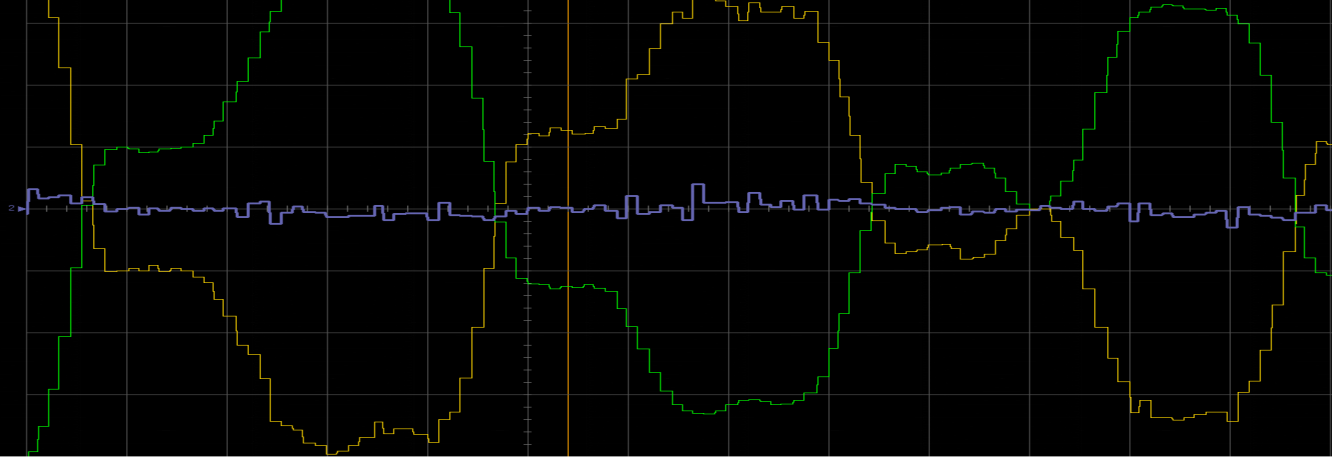
\includegraphics[width=.8\textwidth]{delay.png} 
    \caption{不同通信时延对应的装甲板惯性系下的坐标} 
    \label{delay}
\end{figure}

\section{动态时间帧对齐}[Content specification]

基本思想如下:事先通过上述技术手段测量通信时延。然后以下位机的时钟为基准,下位机定频(100$hz$)向上位机发送本机的时钟信息,上位机将计算本机时钟与下位机时钟之差(在考虑通信时延的情况下),
并将数据放入到循环队列中,当需要在上位机获取下位机时钟时刻时,
通过计算循环队列的平均值作为上下位机时钟偏移量加到本机时钟就可以获得下位机的时钟时刻,如图\ref{clock_sync}所示。

\begin{figure}[H]
    \centering
    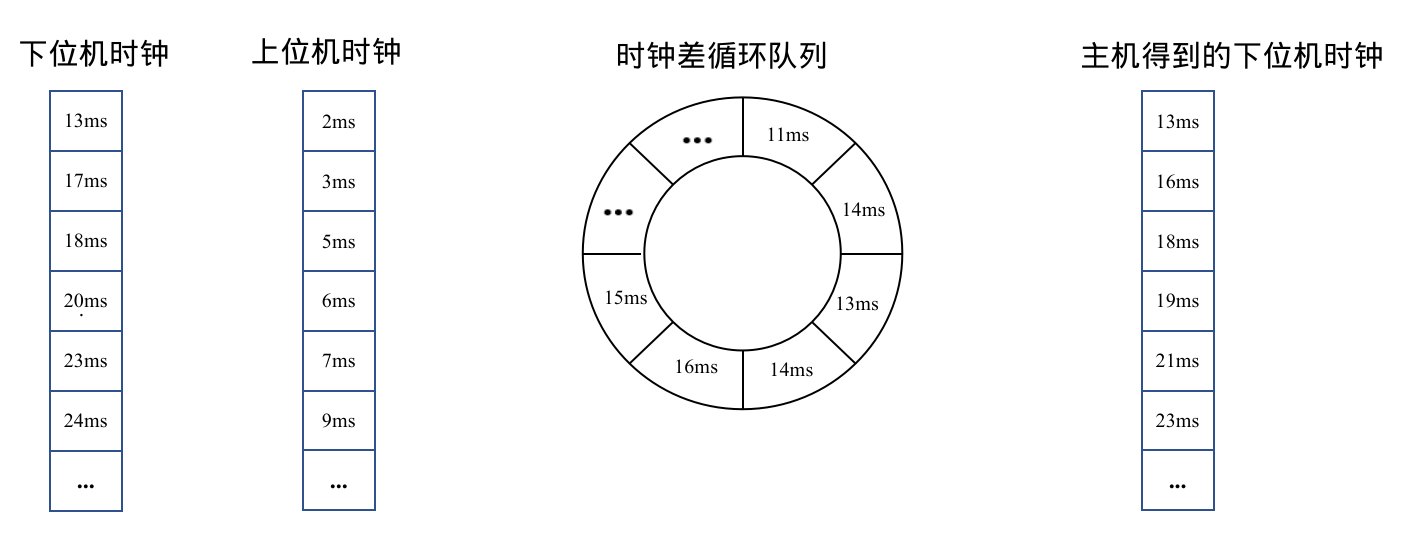
\includegraphics[width=.8\textwidth]{clock_sync.png} 
    \caption{自实现时钟同步} 
    \label{clock_sync}
\end{figure}

% \subsection{线程安全的时间队列}[Content specification]








\section{本章小结}[Content specification]
通过观测固定装甲板惯性下的坐标浮动情况测量通信时延,基于通信实现动态上下位机时间帧对齐,
实现了双机时钟的统一,有利于后续的坐标转换、云台姿态控制等。






